\subsection{\A scaling and speedup}
To measure the speedup caused by the heuristic function, we compare the number
of not only the expanded, but also of explored states (the latter number is
never smaller, and the example in~\cref{TRIEfig:heuristic-benefit}) between
\astarix and \dijkstra on the MHC1 dataset.

\cref{TRIEfig:scaling_with_errors} demonstrates the benefit of the heuristic
function in terms of both alignment time and number of explored states. Most
importantly, \astarix scales much better with increasing number of errors in the
read, compared to \dijkstra. More specifically, the number of states explored by
\dijkstra, as a function of alignment cost, grows exponentially with a base of 
around 10, whereas the base for \astarix is around 3 (the empirical complexity is
estimated as a best exponential fit \mbox{$\mli{exploredStates} \sim a \cdot
\mli{score}^b$}).

The horizontal black line in \cref{TRIEfig:scaling_with_errors} denotes the total
number of states $\lvert \RG \rvert \cdot \lvert q \rvert$, which is always
explored by \bitparallel and \pasgal. On the other hand, any aligner must
explore at least $m = \lvert q \rvert$ states, which we show as a horizontal
dashed line. This lower bound is determined by the fact that at least the states
on a best alignment need to be explored.

\begin{figure}[t]
  \begin{subfigure}{.45\textwidth}
    \centering
    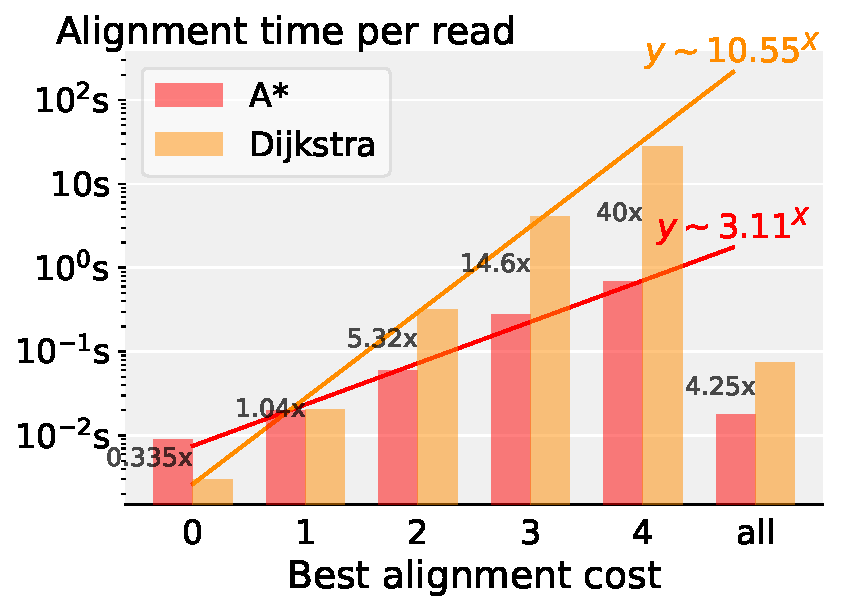
\includegraphics[width=\linewidth]{figs/cmp/heuristic_MHC1_cost-t(map).pdf}
  \end{subfigure}%~\hspace{1em}
  \begin{subfigure}{.45\textwidth}
    \centering
    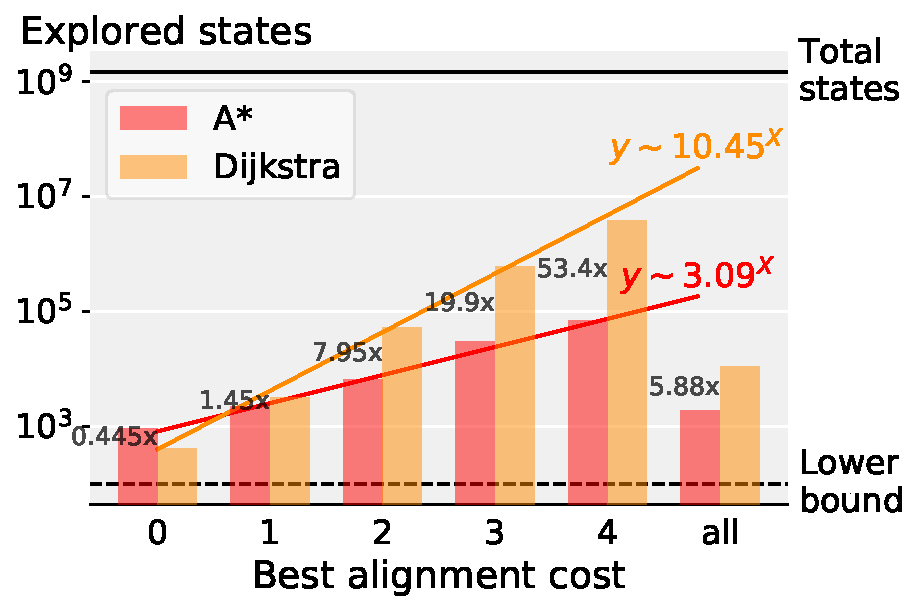
\includegraphics[width=\linewidth]{figs/cmp/heuristic_MHC1_cost-explored_states.pdf}
  \end{subfigure}%
  \caption[Performance scaling with alignment cost]{Comparison of \A and \dijkstra in terms of mean alignment runtime per read and mean explored states depending on the alignment cost on MHC1.}
  \label{TRIEfig:scaling_with_errors}
\end{figure}